\documentclass{letnab}


\rhead{Кафедра высшей математики МФТИ}
\lhead{Кратные интегралы и теория поля: экзамен}
\renewcommand{\headrulewidth}{1pt}

\usepackage{hyperref}

\hypersetup{pdfstartview=FitH,  linkcolor=linkcolor,urlcolor=urlcolor, 
	colorlinks=true}

% Цвета для гиперссылок
\usepackage{xcolor}


\definecolor{linkcolor}{HTML}{000000} % цвет ссылок
\definecolor{urlcolor}{HTML}{0000FF} % цвет гиперссылок
\newtheorem{determenition}{Определение}
\newcommand{\p}{\partial}

\begin{document}
	\tableofcontents
	\newpage


\section{Функции, заданные неявно}
\subsection{Основные понятия}
\begin{equation} \label{eq:1}\
f(x,y)=0; 
\end{equation}
$D_{f}=\{(x,y)\in\mathbf{E}^2: f(x,y)=0 \} $  - график уравнения \ref{eq:1}. $D_f \leftrightarrow Ox$


\begin{minipage}{100mm}
	\subsubsection{Примеры}
	\begin{enumerate}
		\item $x^2+y^2-1=0$ \\
		$f_x=2x; \; f_y=2y$ \\
		Точку (0,1), например, нельзя рассматривать как y=f(x), но можно как x=f(y)
		\item$ (x-y)(x+y-1)=0$ \\
		$f_x=(x+y-1)+(x-y); \;\; f_y=-(x+y-1)+(x-y)$
		$(\frac 1 2;\frac 1 2)$ - особая точка, где обе 0.  Ни по Ox, ни по Oy нет биекции.
	\end{enumerate}
\end{minipage}
\begin{minipage}{70mm}
	\begin{figure}[H]
		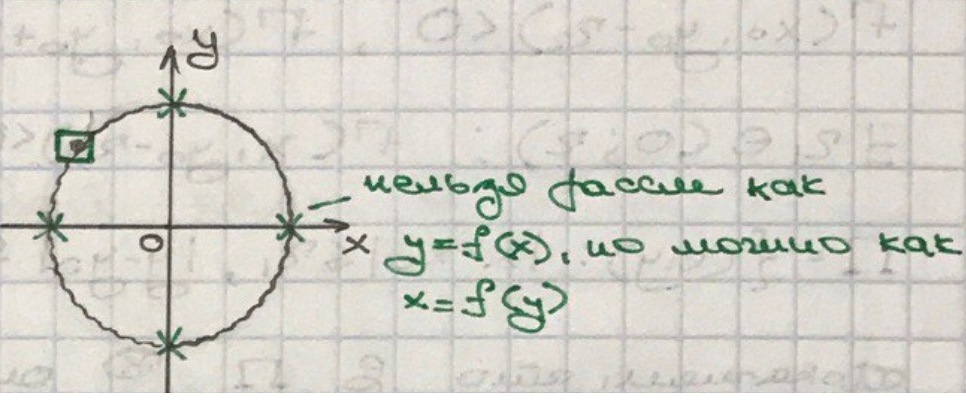
\includegraphics[width=50mm]{lect1pic1}
		\\
		\\
		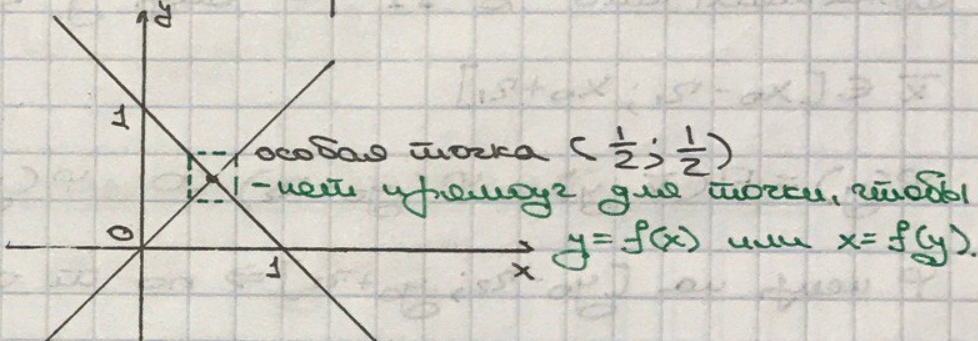
\includegraphics[width=50mm]{lect1pic2}
		\\
	\end{figure}
\end{minipage}

\subsection{Теорема о неявно заданной функции}
Достаточное условие, при котором уравнение \ref{eq:1} локально определеяет y как $f(x)$ и y обладает некоторыми дифф. свойствами.

\begin{theorem}
	Если \begin{enumerate}
		\item $f(x_0,y_0)=0$ \label{enum:1}
		\item в некоторой $u(x_0,y_0)$ функция f обладает непрерывной частной производной\label{enum:2}
		\item $f_y(x_0,y_0)\ne0,$ \label{enum:3}
	\end{enumerate}
То $\exists \Pi=\{(x,y): |x-x_0|\leq r_1, |y-y_0|\leq r_2\} \in U(x_0,y_0)$ в пределах которого уравнение \ref{eq:1} определяет y как функцию переменной x $(y=f(x))$, которая непрерывно дифференцируема на $(x_0-r_1, x_0+r_1)$ и $y'=-\frac{f_x(x,y)}{f_y(x,y)}\left.\right|_{y=f(x)}$
\end{theorem}
\begin{proof}
\textbf{I. Существование неявно заданной функции}\\
	$\ref{enum:3}\Rightarrow$  Пусть $f_y(x_0,y_0)>0 \; \rightarrow_{(2)} \exists \Pi_1= \{(x,y): |x-x_0|\leq r, |y-y_0|\leq r_2\}\in U(x_0,y_0)$ такой, что $\forall (x.y)\in \Pi_1 \Rightarrow f_y(x,y)>0$ \\
	$\psi(y)=f(x_0,y), \; \psi(y_0)=0, \; \psi $- возрастает на $[y_0-r_2, y_0+r_2]$\\
	$\psi'(y)=f_y(x_0,y)>0, \; \forall y\in [y_0-r_2, y_0+r_2] \Rightarrow \psi(y_0-r_2)<0, \psi(y_0+r_2)>0$\\
	$f(x_0, y_0 - r_2)<0, \; f(x_0,y_0+r_2)>0\\
	\exists r_1\in(0,r): \; f(x,y_0-r_2)<0, f(x,y_0+r_2)>0, \forall x\in[x_0-r, x_0+r] \\ \Pi=\{(x,y): |x-x_0|\leq r_1, |y-y_0|\leq r_2\}\in U(x_0,y_0)$\\
	Покажем, что в $\Pi \ref{eq:1}$ определяет $y$ как функцию от $x$\\
	$\overline{x}\in [x_0-r_1, x_0+r_1]\\
	\phi(y)=f(\overline{x},y), \; \phi(y_0-r_2)<0,\; \phi(y_0+r_2)>0$\\
	$\phi(y)$ непрерывна на $[y_0-r_2;y_0+r_2]\Rightarrow$ по теореме о промежуточном значении $\exists \overline{y} \in (y_0-r_2;y_0+r_2): \phi(\overline{y})=0 $ и эта точна единственная.\\
	$\phi'(y)=f_y(\overline{x},y)>0$ в $\Pi_1\subset\Pi \\
	f(\overline{x},\overline{y})=0 \;\; y=f(x)$\\
\textbf{II.}\\	
	$\Pi_1= \{(x,y): |x-x_0|\leq r_1, |y-y_0|\leq r_2\}$\\
	$(x_0,y_0)\in \Pi, \; f(x_0,y_0)=0, \;(x_0+\Delta x, y_0 + \Delta y)\in \Pi$ и $f(x_0+\Delta x,y_0+\Delta y)=0; \\
	\Delta  f=f(x_0+\Delta x,y_0+\Delta y) - f(x_0, y_0)=0;\\
	\Delta  f=f(x_0+\Delta x,y_0+\Delta y) -f(x_0,y_0+\Delta y)+f(x_0,y_0+\Delta y)-  f(x_0, y_0)=0;\\
	\exists \Theta_1, \Theta_2: 0<\Theta_I<1: \Delta  f=f_x(x_0+\Theta_1\Delta x,y_0+\Delta y)\Delta x +f_y(x_0+\Delta x,y_0+\Theta_2\Delta y)\Delta y=0;$\\
	$$\Delta y=- \frac{f_x(x_0+\Theta_1\Delta x,y_0+\Delta y)}{f_y(x_0+\Delta x,y_0+\Theta_2\Delta y)}\Delta x \Rightarrow |\Delta y|\leq \frac{M}{m}|\Delta x| $$
	$\Rightarrow$ при $\Delta x\rightarrow0, \Delta y \rightarrow 0\;\; f_y$ непрерывно в $\Pi$ - компакт  $\Rightarrow \exists m>0: f_y(x,y)\geq m; \;\exists M>0: |f_y(x,y)|\leq M  $ на  $\Pi$ 
	$$\frac{\Delta y}{\Delta x}=-\frac{f_x(x_0+\Theta_1\Delta x, y_0+\Delta y )}{f_y(x_0,y_0+\Theta_2\Delta y)}; \;\;
	f'(x_0)=-\frac{f_x(x_0,f(x_0))}{f_y(x_0,f(x_))};\;\; y_0=-f(x_0);$$
	В силу произвольности $(x_0,y_0)$ производная существует на всем $(x_0-r_1, x_0+r_1)$
\end{proof}
\textbf{Замечание}\\
Теорема остается справедливой, если в $f(x,y)=0, \; x=(x_1,x_2,\dots, x_m)$\\
$\Pi=\{(x_1,x_2,\dots, x_m,y): |x_i-x^0_i|_{i=\overline{1,m}}\leq r_i, |y-y_0|\leq \rho \}$

\subsection{Неявные функции, определяемые системой уравнений}
$$\left\{
\begin{aligned}\label{al:1}
f_1(x_1, \dots, x_n, y_1, \dots y_n )=0\\
f_2(x_1, \dots, x_n, y_1, \dots y_n )=0\\
\dots \\
f_n(x_1, \dots, x_n, y_1, \dots y_n )=0\\
\end{aligned}
\right.
$$\\
$x^0\in\mathbb{E}^m, y^0 \in \mathbb{E}^n; \; 
 \Pi(x^0)=\{x\in \mathbb{E}^m: |x_i-x_i^0|\leq r_i, i=\overline{1,m}\}$ \\
$\Pi(y^0)=\{y\in \mathbb{E}^n: |y_i-y_i^0|\leq \rho_i, i=\overline{1,n}\}$ \\
$\Pi=\Pi(x^0)\times \Pi(y_0)=\{(x,y)\in \mathbb{E}^n+m: x\in\Pi(x^0), y\in \Pi(y^0)\}$\\
Система  определяет в $\Pi\; y_1,\dots,y_n$ как неявные функции переменных $x_1, \dots x_m$, если $\forall x \in \Pi(x^0)$ ставится в соответствие такое $y\in \Pi(x^0),$ что $f_i(x,y)=0, \; i\in\overline{1,n}$ 
\begin{theorem}
	Пусть 
	\begin{enumerate}
		\item $f_i(x^0,y^0)=0, \;i\in\overline{1,n}$
		\item Функции $f_i, i\in\overline{1,n}$ обладают в некоторой окрестности $U(x^0,y^0) $ непрерывностью частных проихводных по переменным $x_j, j\in\overline{1,m}$ и $y_i, i\in\overline{1,n}$ 
		\item 
		$\begin{vmatrix}
			\frac{\partial f_1}{\partial y_1} & \dots & \frac{\partial f_1}{\partial y_n}	 \\
			 & \dots & 	 \\
			\frac{\partial f_n}{\partial y_1}& \dots & \frac{\partial f_n}{\partial y_n}
		\end{vmatrix}(x^0,y^0)\ne 0$
	\end{enumerate}
	Тогда $\exists \Pi=\Pi(x^0)\times |pi(y^0) \in U$, в пределах которого система определяет переменные $y_1,\dots,y_n$ как неявно заданные функции переменных $x_1,\dots,x_m$ и эти функции $y_i=f_i(x)$ обладают непрерывными частными производными в $\Pi(x^0)$ и $y^0_i=f'^i(x^0), \overline{1,n}$
\end{theorem}






\section{Локальные экстремумы функций многих переменных}
\subsection{Определение и необходимые условия существования экстремумов}
$\omega=f(x), \; x\in\mathbb{E}^m, \; x=(x_1, x_2, \dots, x_m), x^0=(x^0_1, \dots, x^0_m)$
\begin{determenition}
	Точка $x^0$ называется точкой локального минимума [максимума] функции $\omega=f(x), $ если $\exists B_\delta(x^0): \forall x \in B_\delta(x^0) $ выполнено $f(x^0) < f(x)\;\; [f(x^0) > f(x)] $
\end{determenition}
\begin{theorem}[Необходимое условие существования локального экстремума]
	\label{th:1}
	Если функция $\omega=f(x)$ дифференцируема в точке $x^0$ и имеет в этой точке локальный экстремум, и все ее частные производные в этой точке =0 т.е. 
	$$\frac{\p f}{\p x_1}(x_0) = \frac{\p f}{\p x_2}(x_0) = \dots =  \frac{\p f}{\p x_m}(x_0)=0$$
\end{theorem}
\begin{proof}
	Фиксируем $x^0_2, \dots, x^0_m; \; f(x_1,x^0_2, \dots, x^0_m)=f(x_1); \; f'(x^0_1)=\frac{\p f}{\p x_1}(x^0) $. f диф. в точке $x_1^0$ и имеет в ней локальный экстремум. Тогда по теореме Ферма $f'(x^0_1)=0=\frac{\p f}{\p x_1}(x^0)  $. Равенство 0 остальных ч.п. доказывает аналогично.
\end{proof}
\begin{sentence}
	\ref{th:1} - необходимое, но не достаточное условие существования локального экстремума. например: \\
	$\omega=xy; \; (0,0): \frac{\p \omega}{\p x}(0,0)=\frac{\p \omega}{y}(0,0)=0$, но $\nexists B_\delta(0,0): \forall (x,y) \in B_\delta \rightarrow \omega(x,y)>\omega(0,0)=0$ или $\omega(x,y)<\omega(0,0)=0$. Точка $x^0: \frac{\p f}{\p x_1}(x^0)=\dots=\frac{\p f}{\p x_m}(x^0)=0 $ - стационарная точка
\end{sentence}
\begin{theorem_nu}[\textbf{1'}]\label{th:1'}
	Если $\omega=f(x)$ дифференцируема в точке $x^0$ и имеет в этой точке лок. экстремум, то дифференциал $df(x^0)\equiv 0$ относ дифф. независ. перем. $dx_1, \dots dx_m$
\end{theorem_nu}
\begin{proof}
	$df(x^0)=\frac{\p f}{\p x_1}(x^0)dx_1+ \dots + \frac{\p f}{\p x_m}(x^0)dx_m; \;\;\;$ из т.$ 
	\ref{th:1} \Rightarrow df(x^0)=0$
\end{proof}

\subsection{Достаточное условие существования локального экстремума}
$\omega=f(x), \; x^0: \frac{\p f}{\p x_1}(x^0_1) + \dots +  \frac{\p f}{\p x_m}(x^0_m)=0; $ f -дважды непрерывно дифференцируема в точке $x^0$ т.е. $d^2f(x^0)=\sum\limits_{i=1}^{m}\sum\limits_{j=1}^{m}a_{ij}dx_idx_j; \; a_{ij}=a_{ji};$\\
Это квадратичная форма относительно $dx_i, i=\overline{1,m}; \;$ 
$k=k(x)=\sum\limits_{i=1}^{m}\sum\limits_{j=1}^{m}a_{ij}x_ix_j; \; a_{ij}=a_{ji}$
\begin{enumerate}
	\item k(x) - положительно определенная кв. форма: $\forall x\ne 0 \rightarrow k(x)>0$
	\item k(x) - отрицательно определенная кв. форма: $\forall x\ne 0 \rightarrow k(x)<0$
	\item k(x) - положительно полуопредел. кв. форма: $\forall x \rightarrow k(x)\geq0 \;\&\; \exists x\ne 0: k(x)=0$
	\item k(x) - отрицательно полуопредел. кв. форма: $\forall x \rightarrow k(x)\leq0 \;\&\; \exists x\ne 0: k(x)=0$
	\item k(x) - неопределенная кв. форма: $\exists x', x'': k(x')>0 \;\&\; k(x'')<0$
\end{enumerate}
\begin{theorem}
	\label{th:2}
	Пусть $\omega=f(x)$ дважды непрерывно дифференцируема в некоторой окрестности стационарной точки $x^0$. 
	\begin{enumerate}
		\item Если $d^2f(x^0)$ положительно определенная кв. форма, то т $x^0$ - точка лок. min
		\item Если $d^2f(x^0)$ отрицательно определенная кв. форма, то т $x^0$ - точка лок. max
		\item Если $d^2f(x^0)$ неопределенная кв. форма, то т $x^0$ не является точкой лок. экстремума функции
	\end{enumerate}
\end{theorem}
\begin{proof}
	\begin{enumerate}
		\item $f(x)-f(x^0)=df(x^0)+\frac 1 2 d^2f(x^0) + o(\rho^2), \rho\rightarrow0; \; df(x^0)=0$ по т. \ref{th:1'}. $\; dx_1=x_1-x_1^0\; \dots dx_m=x_m-x^0_m; \; \rho=\sqrt{(x_1-x_1^0)^2+ \dots + (x_m-x_m^0)^2}$\\
		$o(\rho^2)\stackrel{\rho\rightarrow 0}{=}\alpha(\rho)\rho^2,\; \alpha(\rho)\xrightarrow{rho\rightarrow 0}0, \; $\\
		Обозначим $h_i=\frac{x_i - x^0_i}{\rho}; i=\overline{1,m}; \; |h_i|\leq1; \; h^2_i+ \dots h^2_m=1; \; h=(h1, \dots, h_m).$ Тогда:\\
		$$f(x)-f(x^0)=\rho^2\left[\frac 1 2 \sum_{i=1}^{m}\sum_{j=1}^{m}a_{ij} h_i h_j + \alpha(\rho)\right] $$
		Функция $k(h)=\sum_{i=1}^{m}\sum_{j=1}^{m}a_{ij} h_i h_j $ - непрерывна на компакте $S=\{ h: h_1^2+ \dots h^2_m=1 \}$ Тогда по 2 теореме Вейерштрасса:\\
		$\exists h'\in S: h'\ne 0, k(h')=\mu>0, \exists \rho'>0: \forall \rho<\rho' \rightarrow |\alpha(\rho)| < \frac \mu 2 \Rightarrow$\\
		$\Rightarrow \forall \rho<\rho' \rightarrow f(x)-f(x^0)>0. \sum_{i=1}^{m}(x_i-x^0_i)^2<\rho^2$
		\item Аналогично 1 пункту
		\item Как и в первом пункте $f(x)-f(x^0)=df(x^0)+\frac 1 2 d^2f(x^0) + o(\rho^2), \rho\rightarrow0; \; df(x^0)=0$ по т. \ref{th:1'}. $\; dx_1=x_1-x_1^0\; \dots dx_m=x_m-x^0_m; \; \rho=\sqrt{(x_1-x_1^0)^2+ \dots + (x_m-x_m^0)^2}$\\
		$o(\rho^2)\stackrel{\rho\rightarrow 0}{=}\alpha(\rho)\rho^2,\; \alpha(\rho)\xrightarrow{\rho\rightarrow 0}0, \; $\\
		$h_i=\frac{x_i - x^0_i}{\rho}; i=\overline{1,m}; \; |h_i|\leq1; \; h^2_i+ \dots h^2_m=1;$
		Тогда $h_i'=\frac{x_i'-x^0}{\rho}, \; h_i''=\frac{x_i'' - x_0}{\rho}; i=\overline{1,m};$\\
		$\exists h'=(h_1', \dots, h_m'), h''=(h_1'', \dots, h_m''): k(h')>0, k(h'')<0\\
		f(x')-f(x^0) =\rho^2\left[\frac 1 2 \sum_{i=1}^{m}\sum_{j=1}^{m}a_{i,j} h_i' h_j' + \alpha(\rho)\right] \Rightarrow \exists \rho': \forall \rho<\rho' \; f(x')- f(x^0)>0 \\
		f(x'')-f(x^0) =\rho^2\left[\frac 1 2 \sum_{i=1}^{m}\sum_{j=1}^{m}a_{i,j} h_i'' h_j'' + \alpha(\rho)\right] \Rightarrow \exists \rho'': \forall \rho<\rho'' \; f(x'')- f(x^0)<0 \\
		$		
	\end{enumerate}
\end{proof}
\begin{sentence}
	\begin{enumerate}
		\item Если $x^0$ - стационарная точка, $\omega=f(x)$ и $d^2f(x^0)$ - положительно [отрицательно] полуопределенная кв. форма, то о существовании локального экстремума нельзя ничего сказать. $\omega=f_1(x,y)=(x-y)^4, \; \omega=f_2(x,y)=x^4+y^4; \; (x^0,y^0)=(0,0)$ - стационарная точка $f_1$ и $f_2$. Тогда:\\
		$df_1=4(x-y)^3(dx-dy);\; d^2f_1=12(x-y)^2(dx-dy)^2;\; d^2f_1(x,x)=0$ - полуопределенная кв. форма. \\
		$df_2=4x^3dx+4y^3dy;\; d^2f_2=12x^2dx^2+12y^2dy^2>0$ везде кроме (0,0) - точки локального минимума функции $f_2;\; f_2(0,0)=0$
		\item Условие $d^2f(x^0)\geq 0\; [d^2f(x^0)\leq 0]$ - необходимое условие локального экстремума. 
		\paragraph{Примеры}
		\begin{enumerate}
			\item $\omega=x^4+y^4-2x^2;\;\; d\omega=(4x^3-4x)dx+4y^3dy; \;\; d^2\omega=(12x^2-4)dx^2+12y^2dy^2$\\
			$M_1(0,0), M_2(1,0), M_3(-1,0)$\\
			$d^2\omega(M_1)=-4dx^2<0; \; \forall dx\ne 0 \Rightarrow M_1 - $ локальный max\\
			$d^2\omega(M_2)=8dx^2>0; \;  \forall dx\ne 0 \Rightarrow M_2 - $ локальный min\\
			$d^2\omega(M_3)=8dx^2>0; \;  \forall dx\ne 0 \Rightarrow M_3 - $ локальный min\\
			\item $\omega=\lambda x_1^2+x_2^2+\dots + 2x_2 + \dots +2x_m, \lambda\in \mathbb{R}, \lambda\ne 0$\\
			$\frac{\p \omega}{\p x_1}=2\lambda x_1, \frac{\p \omega}{\p x_2}=2x_2+2, \dots, \frac{\p \omega}{\p x_m}=2x_m+2;$\\
			Стационарная точка M(0,-1,\dots, -1)\\
			$d^2\omega=2\lambda dx_1^2+ 2dx_2^2+ \dots 2dx_m^2;$ Тогда есть два случая:
			\begin{enumerate}
				\item $\lambda>0\; \Rightarrow\; d^2\omega^{(M)}>0 \;\;\forall (dx_1, \dots , dx_m) \ne (0,\dots, 0)$ M - точка лок. min
				\item $\lambda<0\; (dx_1, \dots, dx_m)=(1,0,\dots, 0) \; d^2\omega<0 \\
				(dx_1, \dots, dx_m)=(0,1,0,\dots, 0) \; d^2\omega>0$ локальный  экстремум
			\end{enumerate}
		\end{enumerate}
	\end{enumerate}	
\end{sentence}






\section{Понятие условного экстремума}
\paragraph{Пример}
$\omega=x^2+y^2,	$ при условии $x+y-1=0.$\\
$y=1-x, \omega = x^2+(1-x)^2=2x^2-2x+1$\\
$\omega'=2(2x+1)=0 \Rightarrow x_0=-\frac 1 2$
$\omega''=x>0 \rightarrow x_0$ - локальный минимум $\omega=\omega(x)$\\
$M_0(\frac 1 2; \frac 1 2)$ - т. условного минимума $\omega=x^2+y^2$ при $x+y-1=0; \omega=\frac 1 2$. Абсолютный экстремум $\omega=0$ в (0;0)
\subsection{Общая постановка задачи}
$\omega=f(x,y), \; x\in\mathbb{E}^m, \; y\in\mathbb{E}^n; \; x=(x_1,x_2,\dots, x_m), \; y=(y_1,\dots, y_n);$
\begin{equation}\label{connect}
	\Phi_1(x,y)=0, \; \Phi_2(x,y)=0, \; \dots \Phi_n(x,y)=0;\; \text{  - условия связи}
\end{equation}
Условия связи \ref{connect} в пространстве $\mathbb{E}^{m+n}$ определяют множество $\mathbb{X}:$ $$\mathbb{X}=\{(x,y): \Phi_1(x,y)=0, \; \Phi_2(x,y)=0, \; \dots \Phi_n(x,y)=0 \};\; dim \mathbb{X} = m$$
\begin{determenition}[Точка условного минимума]
	точка $M_0(x^0, y^0): \Phi_i(x^0, y^0)=0, \forall i=\overline{1,n},$ называется точкой лок. min [max] функции $\omega=f(x,y),$ при условиях связи \ref{connect}, если 
	$$\exists B_\varepsilon (M_0):\; \forall (x,y)\in B_\varepsilon (M_0) \cap \mathbb{X} \Rightarrow f(x^0, y^0)<f(x,y) \; [f(x^0, y^0)>f(x,y)]$$
\end{determenition}
\subsection{Необходимые условия существования лок. экстремума}
$M_0(x^0, y^0): \Phi_i(x^0, y^0) = 0, i =\overline{1,n}; \;\; f, \Phi_1, \dots, \Phi_n $ - непр дифф в некоторой окр $U(M_0)$
$$\frac{D(\Phi_1, \dots , \Phi_n)}{D(y_1, \dots, y_n)}=\Delta_{\Phi, y}=
\begin{vmatrix}
\frac{\partial \Phi_1}{\partial y_1}&\dots &  \frac{\partial \Phi_1}{\partial y_n} 	\\ 
\vdots& & \vdots\\
\frac{\partial \Phi_n}{\partial y_1}&\dots & \frac{\partial \Phi_n}{\partial y_n} 
\end{vmatrix}(M_0)\ne 0
$$
$\exists \Pi=\Pi(x^0)\times\Pi(y^0)\subset U(M_0): y_1=\varphi_1(x1,\dots ,x_m) \dots  y_n=\varphi_n(x1,\dots ,x_m)$\\
$\omega)=f(x)=f(x_1,\dots , x_m, y_1, \dots ,y_n)=f(x, \varphi_1(x), \dots \varphi_n(x)$\\
Если $x^0 $- точка лок. экстремума  f, $ \Rightarrow df(x^0) \equiv 0 \; \forall dx_1,\dots, dx_m \Rightarrow \\ 
\Rightarrow df(x^0, y^0)\equiv 0 = \sum\limits_{k=1}^{m} \frac{\partial f}{\partial x_k}(M_0) dx_k + \sum\limits_{j=1}^{n} \frac{\partial f}{\partial y_j}(M_0)dy_j$\\
где $dy_j(M_0) = \sum\limits_{i=1}^{m} \frac{\partial \varphi_j}{\partial x_i}(x_0)dx_i, j=\overline{1,n}$\\
$A_1dx_1+ \dots + A_mdx_m \equiv0 \; \forall dx_1, \dots, dx_m \Rightarrow$ \\
\textbf{Необх. условие существования лок. условного экстремума: $A_1=\dots =A_m=0. $}
\textbf{Замечания:}
\begin{enumerate}
	\item Теорема о функциях, заданных неявно системой уравнений, говорит только о существовании функций $\varphi_1\dots \varphi_n$, но не дает метода их нахождения
	\item В приведенных рассуждениях $x_1, \dots x_m$ - независимые переменные, а $y_1, \dots y_n$ - зависимые
\end{enumerate}
	Если $\varphi_1\dots \varphi_n$ - неизвестны, то  $dy_j(M_0)$ можно найти как:   
	\begin{align}	
	 &\frac{\partial \Phi_1}{\partial x_1}(M_0)dx_1+ \dots + 
	  \frac{\partial \Phi_1}{\partial x_m}(M_0)dx_m+ 
	  \frac{\partial \Phi_1}{\partial y_1}(M_0)dy_1+ \dots
	  \frac{\partial \Phi_1}{\partial y_n}(M_0)dy_n = 0\\ 
	 &\vdots\\
	 &\underbrace{\frac{\partial \Phi_1}{\partial x_1}(M_0)dx_1+ \dots + 
	 \frac{\partial \Phi_1}{\partial x_m}(M_0)dx_m }_{D+\mathbb{J}dy=0} +\frac{\partial \Phi_1}{\partial y_1}(M_0)dy_1+ \dots
 	 \frac{\partial \Phi_1}{\partial y_n}(M_0)dy_n = 0
	\end{align}
\subsection{Метод Лагранжа}
Выполненные условия связи \ref{connect} 
	\begin{multline*}
		\left\{
			\begin{aligned}
				\frac{\partial f}{\partial x_1}(M_0)dx_1+ \dots + 
				\frac{\partial f}{\partial x_m}(M_0)dx_m+ 
				\frac{\partial f}{\partial y_1}(M_0)dy_1+ \dots
				\frac{\partial f}{\partial y_n}(M_0)dy_n = 0
				\\
				D+\mathbb{J}dy=0 \; | \times \lambda=
					\begin{pmatrix}
						\lambda_1 \\ \dots\\ \lambda_n
					\end{pmatrix}
			\end{aligned} 
		\right| + 
		\\
		+\sum\limits_{k=1}^m \left[\frac{\partial f}{\partial x_k}(M_0) + \lambda_1  \frac{\partial \Phi_1}{\partial x_k}(M_0)+ \dots + \lambda_n  \frac{\partial \Phi_n}{\partial x_k}(M_0)\right]dx_k+ 
		\\
		+\sum\limits_{j=1}^n \left[\frac{\partial f}{\partial y_j}(M_0) + \lambda_1  \frac{\partial \Phi_1}{\partial y_j}(M_0)+ \dots + \lambda_n \frac{\partial \Phi_n}{\partial y_j}(M_0)\right]dy_j=0
	\end{multline*}
$\lambda_1, \dots, \lambda_n $ выбираются таким образом, чтобы \\
\begin{equation}\label{lambda0sist2}
	\left\{ \begin{array}{rcl}
		&\frac{\partial f}{\partial y_1}(M_0) + \lambda_1  \frac{\partial \Phi_1}{\partial y_1}(M_0)+ \dots + \lambda_n  \frac{\partial \Phi_n}{\partial y_1}(M_0)
		\\ &\dots \\
		&\frac{\partial f}{\partial y_n}(M_0) + \lambda_1  \frac{\partial \Phi_1}{\partial y_n}(M_0)+ \dots + \lambda_n  \frac{\partial \Phi_n}{\partial y_n}(M_0)
	\end{array}\right.
\end{equation}
	
\begin{equation}\label{lambda0sist2'}
\left[ \frac{\partial \Lambda}{\partial x_k}(M_0) = 0, \; k=\overline{1,m}    \right]
\end{equation}
$\exists! \; \lambda^0=(\lambda^0_1, \dots, \lambda_n^0);$\\
Подставляем $\lambda_0: \; 
\sum\limits_{k=1}^m \left[\frac{\partial f}{\partial x_k}(M_0) + \lambda^0_1  \frac{\partial \Phi_1}{\partial x_k}(M_0)+ \dots + \lambda^0_n  \frac{\partial \Phi_n}{\partial x_k}(M_0)\right]dx_k=0$

\begin{equation}\label{lambda0sist1}
	\left\{ \begin{array}{rcl}
		&\frac{\partial f}{\partial x_1}(M_0) + \lambda_1^0  \frac{\partial \Phi_1}{\partial x_1}(M_0)+ \dots + \lambda_n^0  \frac{\partial \Phi_n}{\partial x_1}(M_0)
		\\ &\dots \\
		&\frac{\partial f}{\partial x_m}(M_0) + \lambda_1^0  \frac{\partial \Phi_1}{\partial x_m}(M_0)+ \dots + \lambda_n  \frac{\partial \Phi_n}{\partial x_m}(M_0)
	\end{array}\right.
\end{equation}

\begin{equation}\label{lambda0sist1'}
\left[ \frac{\partial \Lambda}{\partial y_j}(M_0) = 0, \; j=\overline{1,n}    \right]
\end{equation}
В итоге из этого всего имеем 2n+m уравнений для нахождения $(x_1, \dots, x_m, y_1, \dots, y_n, \lambda_1, \dots,  \lambda_n)$
\\
\begin{theorem}[необходимое условие существования локального экстремума]\label{musthavelocal}
	Пусть функции $f, \Phi_1, \dots, \Phi_n$ непрерывно дифф. в $U(M_0)$, $\Delta_{\Phi, y}\ne0$, и $M_0(x_0, y_0)$ - т. локального условного экстремума функции $\omega=f(x,y)$ при условиях связи $\Phi_1(x,y)=0, \dots, \Phi_n(x,y)=0 $\\ 
	Тогда найдутся числа $(\lambda_1^0, \dots, \lambda_n^0)=\lambda^0$ такие, что в точке $M_0$ выполнены \ref{lambda0sist1} и \ref{lambda0sist2}\\
	$\Lambda(x,y,\lambda)=f(x,y)+\lambda_1\Phi_1(x,y)+\dots + \lambda_n\Phi_n(x,y)$ - функция Лагранжа
\end{theorem}
\textbf{Следствие:}\\
Пусть выволнены условия теоремы \ref{musthavelocal}. Если т $M_0$ является точкой локального условного экстремума функции $\omega=f(x, y)$ при условии связи $\Phi_1(x,y)=0, \; \dots \Phi_n(x,y)=0;$ то в ней выполнены равенства \ref{lambda0sist1'} и \ref{lambda0sist2'}, т.е. $M_0$ - стационарная точка функции Лагранжа.

\subsection{Достаточные условия существования локального экстремума}
$\Lambda(x,y,\lambda) = f(x,y)+ \lambda_1\Phi(x,y)+ \dots + \lambda_n\Phi_n(x,y);\\
\lambda^0=(\lambda_1^0, \dots,\lambda_1^0);\;\; x^0=(x_1^0,\dots,x_m^0);\;\; y^0=(y_1^0,\dots,y_n^0)$
\begin{equation}
	\left\{ \begin{array}{rcl}
		&\frac{\partial \Lambda}{x_k}=0		&k=\overline{1,m}\\
		&\frac{\partial \Lambda}{y_j}=0		&j=\overline{1,n}\\
		&Q\Phi_i=0;\; 						&i=\overline{1,n}
	\end{array}\right.
\end{equation}
$f, \Phi_1,\dots, \Phi_n$ дважды непрерывно дифференцируемы в $U(M_0), \; \Delta_{\Phi, y}(M_0)\ne 0;\; M_0(x^0, y^0)\in X, \; M(x^0+\Delta x, y^0+ \Delta y)\in X\\
\Delta f(M_0, (\Delta x, \Delta y))= f(M)-f(M_0)=\Lambda(M, \lambda^0) - \Lambda(M_0, \lambda^0)=\Delta \Lambda(M_0, \lambda^0, \Delta x, \Delta y)  $
\begin{multline*}
	\Delta\Lambda\left(M_0,(\Delta x, \Delta y)\right) = 
\\ = \frac 1 2 
	\left[
		\sum\limits_{k,j=1}^{m} \frac{\partial^2\Lambda(M_0)}{\partial x_k\partial x_j}  \Delta x_k \Delta x_j + 
		\sum\limits_{k=1}^{m}\sum\limits_{j=1}^{n} \frac{\partial^2\Lambda(M_0)}{\partial x_k\partial y_j}  \Delta x_k \Delta y_j + 
		\sum\limits_{k,j=1}^{n} \frac{\partial^2\Lambda(M_0)}{\partial y_k\partial y_j}  \Delta y_k \Delta y_j
	\right] +
\\ +
		\sum\limits_{k,j=1}^{m} \alpha_{kj}^1  \Delta x_k \Delta x_j + 
		\sum\limits_{k=1}^{m}\sum\limits_{j=1}^{n} \alpha_{kj}^2  \Delta x_k \Delta y_j + 
		\sum\limits_{k,j=1}^{n} \alpha_{kj}^3 \Delta y_k \Delta y_j = 
\\ 	=
	\left/ \begin{array}{rcl}
		&\alpha_{kj}^i\rightarrow 0	&\text{ при }	\Delta x \rightarrow 0;\;\; \alpha_{kj}^2, \alpha_{kj}^3 \text{ зависят от } \Delta x, \Delta y
		\\
		&\Delta y_j \rightarrow 0 &\text{ при } \Delta x \rightarrow 0;\; j=\overline{1,n}  \\
		&\Delta x_j = dx_j;\; \Delta y_j=\alpha y_j+ \gamma_j, \gamma \rightarrow 0  	&\text{ при }	\Delta x \rightarrow 0;\; j=\overline{1,n}
	\end{array}\right/=
\\	= 
		\frac 1 2 
		\left[
		\sum\limits_{k,j=1}^{m} \frac{\partial^2\Lambda}{\partial x_k\partial x_j}  d x_k d x_j + 
		\sum\limits_{k=1}^{m}\sum\limits_{j=1}^{n} \frac{\partial^2\Lambda}{\partial x_k\partial y_j}  d x_k d y_j + 
		\sum\limits_{k,j=1}^{n} \frac{\partial^2\Lambda}{\partial y_k\partial y_j}  d y_k d y_j
		\right] + 
\\ +
		\sum\limits_{k,j=1}^{m} \widetilde{\alpha_{kj}^1}  d x_k d x_j + 
		\sum\limits_{k=1}^{m}\sum\limits_{j=1}^{n} \widetilde{\alpha_{kj}^2}  d x_k d y_j + 
		\sum\limits_{k,j=1}^{n} \widetilde{\alpha_{kj}^3} d y_k d y_j
\end{multline*}
$dy_j (M_0) = \sum\limits_{k=1}^m C_k dx_k;\; d^2\widetilde{\Lambda}(M_0, (\Delta x, \Delta y))= \sum\limits_{k,j=1}^m A_{kj} dx_k dx_j; \; A_{kj}=A_{jk}$\\
$\Delta =\Lambda(M_0,(\Delta x, \Delta y))=d^2\hat{\Lambda}(M_0)+\beta(\Delta x), \; \beta(\Delta x) \rightarrow 0 $ при $\Delta x\rightarrow 0$ \\
$d^2\hat{\Lambda}(M_0)=d^2\Lambda(M_0)$  т.к. первые производные функции Лагранжа в стационарной точке $M_0 ;\;\; =0 \; \Rightarrow d^2y $ равны 0\\
\\
\begin{theorem}
	Пусть f и $\Phi_j, j=\overline{1,n}$ дважды дифф функции в $U(M_0)$ ($M_0$ - стационарная точка функции Лагранжа) и $\Delta_{\Phi, y}(M_0)\ne 0 $ тогда
	\begin{enumerate}
		\item Если $d^2\hat{\Lambda}(M_0)$ положительно определенная квадратичная форма, то $M_0$ - точка условного минимума  функции f при условии связи
		\item Если $d^2\hat{\Lambda}(M_0)$ отрицательно определенная квадратичная форма, то $M_0$ - точка условного максимума функции f при условии связи
		\item Есои $d^2\hat{\Lambda}(M_0)$ неопределенная квадратичная форма, то экстремума нет
	\end{enumerate}
\end{theorem}
\textbf{Замечание:} если $d^2\hat{\Lambda}(M_0)$ полуопределенная кв. форма, то нужно проводить дополнительные исследования

\documentclass{letnab}
\usepackage{amsmath}
\usepackage[english,russian]{babel}
\usepackage{indentfirst}
\usepackage{amssymb}
\usepackage{amsfonts}
\usepackage{amsthm}
\usepackage[T2A]{fontenc}
\usepackage[utf8]{inputenc}
\usepackage{epigraph}
\usepackage{tikz}

\rhead{Кафедра высшей математики МФТИ}
\lhead{Кратные интегралы и теория поля: экзамен}
\renewcommand{\headrulewidth}{1pt}

\usepackage{hyperref}

\hypersetup{pdfstartview=FitH,  linkcolor=linkcolor,urlcolor=urlcolor, 
	colorlinks=true}

% Цвета для гиперссылок
\usepackage{xcolor}


\definecolor{linkcolor}{HTML}{000000} % цвет ссылок
\definecolor{urlcolor}{HTML}{0000FF} % цвет гиперссылок
\newtheorem{determenition}{Определение}
\newcommand{\p}{\partial}
\begin{document}

\section{Кратные интегралы}\vspace{-10pt}
\subsection{Определения и свойства}
\begin{determenition}\vspace{-10pt}
	Совокупность измеримых открытых множеств $T=\{\Omega_k \}_{k=1}^n $ называется разбиением множества $\Omega$, если:
	\begin{enumerate}\vspace{-10pt}
		\item $\Omega_k\subset \Omega, \; k=\overline{1,n} $\vspace{-10pt}
		\item $\Omega_k\cap \Omega_j = \emptyset $, если $k\ne j $\vspace{-10pt}
		\item $\cup_{k=1}^n \overline{\Omega}_k = \overline{\Omega}$
	\end{enumerate}
\end{determenition}

\begin{determenition}\vspace{-10pt}
	$\Delta(\Omega)=\sup_{x,y\in \Omega}\rho(x,y)$ - диаметр множества. ($\Omega  $ - огранич. мн-во)
\end{determenition}

\begin{determenition}\vspace{-10pt}
	Число $\Delta_T=\max_{1\leq k \leq n} \Delta(\Omega_k) $ - называется  мелкостью разбиения $T=\{\Omega_k\}_{k=1}^n$ 
\end{determenition}

\begin{determenition}\vspace{-10pt}
	Разбиение $T'=\{\Omega_j'\} $ - называется измельчением разбиения $T=\{\Omega_k\}$ если $\forall \Omega_j'\subset T \;\; \exists \Omega_k\subset T: \Omega'_j\subset \Omega_k $
\end{determenition}

\paragraph{Свойства измельчения:}\vspace{-10pt}
\begin{enumerate}\vspace{-10pt}
	\item Если $T'$ измельчение $T$, а $T''$ - измельчение $T'$ то $T'$ измельчение $T''$\vspace{-10pt}
	\item Для двух разбиений $T'=\{\Omega_k'\}$ и $T''=\{\Omega_j''\}$ множества $\Omega \;$  $\exists $ разбиение $T $ множества $\Omega \;$, что Т будет измельчением разбиений $T'$ и $T''$
\end{enumerate}

\paragraph{Замечание:}\vspace{-10pt}
	Если $G=\cup^p_{j=1} Q_j $ клеточное множество и $\Omega \subset G $  то в качестве разбиения множества $\Omega $ можно взять $T=\{\Omega_k \} $, где $\Omega_k = \Omega\cap int(Q_k), \; k=\overline{1,p} $

\subsection{Интегральные суммы. Кратный интеграл Римана. \\Необходимое усл. существования кр. интеграла Римана}
$T=\{\Omega_k \}_{k=1}^n,  \omega=f(x), x\in \mathbb{E}$, опред. на $\overline{\Omega}; \;\;\xi = \{\xi_1, \dots, \xi_n \}: \xi \in \overline{\Omega_k} $

\begin{determenition}\vspace{-10pt}
	$I\{T, \xi\} = \sum\limits_{k=1}^n f(\xi_k)m(\Omega_k) - $ интегральная сумма функции $f$
\end{determenition}

\begin{determenition}\vspace{-10pt}
	$m(\Omega_k)$ - мера множества $ \Omega_k$
\end{determenition}


\begin{determenition}\vspace{-10pt}
	Число $I$ называется пределом интегральных сумм $I\{T,\xi \} $, при мелкости разбиения стремящейся к 0, если:\vspace{-10pt}
$$\forall \varepsilon>0 \exists \delta=\delta(\varepsilon)>0: \; \forall T: \Delta_T< \delta\;\&\; \forall \varepsilon \Rightarrow  |I\{T,\xi \} - T|< \varepsilon$$
\end{determenition}

\begin{determenition}[Кратный интеграл Римана]\vspace{-10pt}
	Число $I $, являющееся пределом интегральных сумм при $\Delta_t\rightarrow 0$ называется кратным интегралом Римана функции $f$ по множеству $\Omega \; [\;\overline{\Omega}\;]$. А функция $f$ называется интегрируемой по риману по множеству $\Omega \; [\;\overline{\Omega}\;].$
\end{determenition}\vspace{-20pt}
\vspace{-10pt}
\paragraph{Обозначение:} $\int\limits_\Omega f(x) d\omega = \int...\int_\Omega f(x_1, \dots, x_m) dx_1\dots dx_m =\int...\int_\Omega f dx_1\dots dx_m   $
\begin{theorem}\vspace{-5pt}
	Пусть $\Omega\subset \mathbb{E}^mf $ - измеримая область, а $\omega = f(x)  $ опред. и инт. на $\overline{\Omega} $ тогда эта функция ограничена на $\overline{\Omega} $
\end{theorem}

% А эта теорема вообще нужна? %
\vspace{-10pt}
\paragraph{Пример:} $\omega=f(x)\equiv c; \; \forall x\in \overline{\Omega}, \; \Omega $ - измеримое множество. \\
$\forall T=\{\Omega_k  \}_{k=1}^n \; \forall \xi \;\; I=\{T, \xi \}= \sum_{k=1}^n C\cdot m(\Omega_k) =  C\cdot m(\Omega)$
\vspace{-10pt}
\begin{theorem}
	 Пусть $\Omega\subset \mathbb{E}^m $ - измеримая область, $\omega=f(x)  $ опр. и огр на $\overline{\Omega}. \;\; f(x)\equiv 0 $ на $\overline{\Omega}\backslash \Gamma, \; m(\Gamma)=0, $ тогда f интегрируема на $\Omega$ и $\int_\Omega fd\omega=0 $
\end{theorem}\vspace{-20pt}\begin{proof}
	$\exists c>0 : \forall x\in \overline{\Omega} \rightarrow |f(x)|\leq c $\\
	$\forall \varepsilon>0 \exists G_\varepsilon= \cup_{j=1}^p Q_j : \Gamma \subset G_\varepsilon  $ и $0\leq m\Gamma \leq m(G_\varepsilon) < \frac{ \varepsilon}{c} $\\
	$T=\{\Omega_k  \}_{k=1}^n, \widetilde{T}=T'\cup T'' = \{\Omega_k' \}\cup\{\Omega_j'' \}; \;$  где $\Omega_k'=\Omega_k\backslash \overline{G_\varepsilon}   $ и $\Omega_j''= \Omega_j\cap (int (Q_i)), i=\overline{1,p}, j= \overline{1,n}.$  
	И т.к. на $\Omega_k' $ функция $f(x)\equiv0$, а $\Omega_j'' $ содержит точки из $\Gamma$ получим:\\
	$\forall \xi \rightarrow |I\{\widetilde{T}, \xi \}|= |\sum_j f(\xi_i)m (\Omega_j'') |\leq c\cdot m(G_\varepsilon) < c\cdot \frac{\varepsilon}{c} = \varepsilon $
\end{proof}\vspace{-30pt}
\subsection{Суммы Дарбу. критерий интегрируемости.\\ Интеграл непрерывных функций}

$\Omega \subset \mathbb{E}^m $ измеримая область. $\omega=f(x) $ определена и ограниченна на $\overline{\Omega}.\; T=\{\Omega_k \}_{k=1}^n $ - разбиение $\Omega$. $m_k=\inf_{x\in \overline{\Omega}_k} f(x) , M_k=\sup_{x\in \overline{\Omega}_k} f(x)$\\
$S_*(T)=\sum_{k=1}^n m_k m(\Omega_k); \; S^*(T)=\sum_{k=1}^n M_k m(\Omega_k); \;  $ - \textbf{ нижняя и верхняя  суммы Дарбу}
 
\begin{theorem}[Критерий интегрируемости]
	Пусть $\omega\subset \mathbb{E}$ - измеримая область, а функция $\omega=f(x)$ опр. и огр. на $\overline{\Omega}$. Для того, чтобы $f $ была интегрируема на $\Omega$ необходимо и достаточно чтобы $\boxed{\forall \varepsilon>0\; \exists T: |S^*(T) - S_*(T)|<S |} $
\end{theorem}

\begin{theorem}[Интегрируемость функции, непрерывной на замкнутом измеримом мн-ве]
	Функция $\omega=f(x)$ непр. на замыкании измеримой области $\Omega $ интегрируема на ней.
\end{theorem}




% доказательств на лекции не было. А они нужны вообще?%






\end{document}
\documentclass{letnab}
\usepackage{amsmath}
\usepackage[english,russian]{babel}
\usepackage{indentfirst}
\usepackage{amssymb}
\usepackage{amsfonts}
\usepackage{amsthm}
\usepackage[T2A]{fontenc}
\usepackage[utf8]{inputenc}
\usepackage{epigraph}
\usepackage{tikz}

\rhead{Кафедра высшей математики МФТИ}
\lhead{Кратные интегралы и теория поля: экзамен}
\renewcommand{\headrulewidth}{1pt}

\usepackage{hyperref}

\hypersetup{pdfstartview=FitH,  linkcolor=linkcolor,urlcolor=urlcolor, 
	colorlinks=true}

% Цвета для гиперссылок
\usepackage{xcolor}


\definecolor{linkcolor}{HTML}{000000} % цвет ссылок
\definecolor{urlcolor}{HTML}{0000FF} % цвет гиперссылок
\newtheorem{determenition}{Определение}
\newcommand{\p}{\partial}
\begin{document}

\section{Свойства кратных интегралов}
\begin{theorem}
	Если $\Omega\subset\mathbb{E}^m$ - измеримая область, то $\int_\Omega= m(\Omega) $
\end{theorem}\vspace{-15pt}
	$f(x)\equiv 1 $ на $\overline{\Omega} .  \forall x\in \overline{\Omega}, \; \Omega $ - измеримое множество.
\begin{theorem}[интегрируемость подмнож.] \label{th6.2}
	Пусть $\Omega\subset\mathbb{E}^m$  и  $\Omega'\subset \Omega$ измеримые области и функция $\omega=f(x)$  интегрируема на $\Omega$ , тогда $f$ интегрируема на множестве $\Omega'$
\end{theorem}\vspace{-15pt}
\begin{proof}
	$\Omega'\ne \Omega;\; f$ интегрируема на $\Omega.$ 
	$T=\{\Omega_k\}, T'=\{\Omega_k'\}  $, где $\Omega_k'=\Omega_k\cap \Omega' $ тогда
	$ \;\; \forall \varepsilon>0 \; \exists T: S^*(T)-S_*(T) < \varepsilon;\; $\\
	$M_k'=\sup_{\overline{\Omega}_k'}f \leq \sup_{\overline{\Omega}_k} f = M_k; m_k'=\inf_{\overline{\Omega}_k'}f \geq \inf_{\overline{\Omega}_k} f = m_k \Rightarrow$
	
	\begin{equation} \label{eq6.2}
		 S^*(T')-S_*(T')\leq S^*(T)-S_*(T)<\varepsilon\; 
	 \end{equation}
\end{proof}\vspace{-10pt}

\begin{theorem}[аддитивность интеграла]
	Пусть $\Omega$ и $\Omega'$ измеримые области в $\mathbb{E}^m,\; \Omega'\subset\Omega$ и $ \Omega''=\Omega\backslash \overline{\Omega}'.$ Если функция $\omega=f(x)$ интегрируема на $\Omega $, то $f$ интегрируема на   $\Omega' $ и $\Omega'' $ и $ \int_\Omega fd\omega = \int{\Omega'}fd\omega + \int{\Omega''}fd\omega $
\end{theorem}
\begin{proof} \vspace{-15pt}
	Из теоремы \ref{th6.2} $\Rightarrow \; f$ интегрируема на $\Omega' $ и $\Omega'' $ и существует интеграл в \ref{eq6.2}. $T'$ - разбиение $\Omega' $. $T''$ - разбиение $\Omega''$.  Тогда $T=T'\cup T''$ -разбиение множества $\Omega$. \\
	$\Delta_t= \max\{\Delta_{T'}, \Delta_{T''} \}.\; \forall \xi', \xi'': \xi=\xi'\cup \xi'' \rightarrow I\{T, \xi\}= I\{T', \xi'\}+ I\{T'', \xi''\}  $
	$\Delta_T \rightarrow 0 \Rightarrow \ref{eq6.2}$
\end{proof}

\begin{theorem}[линейность интеграла]
	Пусть $\Omega\subset \mathbb{E}^m$ измеримая область. $\omega=f(x)$  и $\omega=g(x)$ интегрируемые на $\Omega$ функции. Тогда $\forall \alpha, \beta\in\mathbb{R} $ функция $\omega= \alpha f(x) + \beta g(x) $ интегрируема на $\Omega$: \\
	$\int_\Omega \big[\alpha f + \beta g \big]d\omega = \alpha \int_\Omega fd\omega + \beta \int_\Omega gd\omega$  \\
	Кроме того функция $\omega=f\cdot g $ так же интегрируема на $\Omega$ 
\end{theorem}

\begin{theorem}[Инт. от положительной функции]
	Пусть $\Omega\subset \mathbb{E}^m$ измеримая область. Функция $\omega=f(x)$ определена на $\overline{\Omega}, \; f(x)\geq 0 \forall x\in \Omega$ и $f$ интегр на $\Omega$. Тогда: $\int_\Omega fd\omega\geq 0  $
\end{theorem}

\begin{theorem}
	Если $f$ и $g$ интегрируема на измеримой области $\Omega \subset \mathbb{E}^m $ и $\forall x\in \overline{\Omega} \rightarrow f(x) \geq g(x), $ то $ \int_\Omega fd\omega\geq \int_\Omega gd\omega$ 
\end{theorem}

\begin{theorem}
	Если $f$  интегрируемость на измеримой области $\Omega \subset \mathbb{E} $, то функция $|f|$ интегрируема на $\Omega$ и выполнено: $|\int_\Omega fd\omega|\leq \int_\Omega|f|d\omega \leq cm(\Omega),  $ где $c:\forall x\in \overline{\Omega} \rightarrow |f(x)|\leq c $
\end{theorem}

\paragraph{Замечание:}\vspace{-10pt}
В обратную сторону не верно. Контрпример - функция Дирихле.

\begin{theorem}
	Если $\Omega\subset \mathbb{E}$ и $\Omega'\subset \mathbb{E}: \Omega'\subset \Omega, \omega=f(x) $ интегрируема на $\Omega$ и $f(x)\geq 0 \;\forall x\in\ \Omega,$ тогда $\int_{\Omega'}fd\omega \leq \int_\Omega f d\omega $
\end{theorem}

\begin{theorem}
	Пусть функции $\omega=f(x) $ и  $\omega=g(x) $ интегрируемы на измеримой области $\Omega\subset \mathbb{E}$. $g$ не меняет знак на $\overline{\Omega},\; m\leq f(x) \leq M\; \forall x \in \overline{\Omega},$ тогда $\exists \mu: m\leq \mu \leq M:  \int_\Omega fgd\omega = \mu \int_\Omega gd\omega.\;\; $	Если  же $f$ непрерывна на $\overline{\Omega}$, то $\exists x^0 \in \overline{\Omega}:  \int_\Omega fgd\omega = f(x^0) \int_\Omega gd\omega$ 
\end{theorem}

\begin{theorem}
	Пусть $\Omega\subset \mathbb{E}^m$ - измеримая область $\Omega_1 \subset  \Omega_2 \subset  \Omega_3 \dots \subset \Omega$ 
\end{theorem}
\begin{proof}
	$\forall x\in \overline{\Omega} \rightarrow |f(x)|\leq C, \widetilde{\Omega}_k=\Omega\backslash \overline{\Omega}_k  $ - измеримое множество и $m(\widetilde{\Omega}_k)=m(\Omega)\backslash m(\overline{\Omega})\backslash m(\overline{\Omega})\xrightarrow{k\rightarrow \infty} 0  \Leftrightarrow  \forall \varepsilon>0 \; \exists k_0: m(\widetilde{\Omega}_{k_0})< \frac{\varepsilon}{4c}$ \\
	$\Omega_{k_0}, f $ интегрируема на $\Omega_{k_0} \Rightarrow \exists T^{k_0} $ область $\Omega_{k_0}: S^*(T^{k_0}) - S_*(T^{k_0})< \frac \varepsilon 2 $\\
	$\exists T=T^{k_0} \cup \widetilde{T}^{k_0}, \;$ где $\widetilde{T}^{k_0} $ разбиение множества $\Omega\backslash \overline{\Omega}_{k_0} = \widetilde{\Omega}_{k_0} $\\
	$S^*(T)-S_*(T)= S^*(T^{k_0}) -  S^*(T^{k_0}) + S^*(\widetilde{\Omega}^{k_0})- S_*(\widetilde{\Omega}^{k_0})< \frac \varepsilon 2 + 2c\frac{\varepsilon}{4c}= \varepsilon $\\
	$|\int_\Omega fd\omega - \int_{\Omega_k} fd\omega| = |\int_{\widetilde{\Omega}}fd\omega|<cm(\widetilde{\Omega})\xrightarrow{k\rightarrow \infty} 0 $
\end{proof}







\end{document}

\section{Сведение кратного интеграла к повторному}
\subsection{Двойные инитегралы}
$\mathbb{E}^2, Oxy, \Pi=\{(x,y): a<x<b, c<y<d \} $
\begin{theorem}
	Пусть функция $\omega=f(x,y) $ определена на $\overline{\Pi}$ и интегрируема на $\Pi$ и выполнено:  $\forall x\in [a,b] \; \exists \; \mathbb{J}(x)=\int_c^d F(x,y) dy $ тогда функция $\mathbb{J}(x)$ интегрируема на $[a,b]$ и существует повторный интеграл: \\
	$$ \int_a^b \mathbb{J}(x)dx = \int_{a}^{b} dx \int_c^d f(x,y) dy \text{ и } \int_a^b dx \int_c^d f(x,y) dy = \iint_\Pi d(x,y) dxdy $$ 
\end{theorem}
\begin{proof}
	$a=x_0<x_1<\dots <x_k=b, \; c=y_0<y_1<\dots < y_n=d$\\
	$\Pi_{ij}=(x_{i-1}, x_{i})\times(y_{j-1}, y_j), i=\overline{1,k}, j=\overline{1,n} $\\
	$\{\Pi_{ij} \} $ - разбиение $\Pi; \; \Delta_x^i=x_i-x_{i-1}, i=\overline{1,k}; \Delta_y^j=y_j-y_{j-1}, j=\overline{1,n}$\\
	$\xi_i\in [x_{i-1}, x_i]  $ в $\overline{\Pi}_{ij}$ выполнено $(inf)\; m_{ij} \leq f(\xi_i, y) \leq M_{ij} \;(sup) $\\
	$\sum_{j=1}^n m_{ij} \Delta^j_y \leq \mathbb{J}(\xi_i)\leq  \sum_{j=1}^n M_{ij} \Delta^j_y  \Rightarrow \\
	\sum_{i=1}^k\sum_{j=1}^n m_{ij} \Delta_y^j \Delta_x^i \leq \sum_{i=1}^k\mathbb{J}(\xi_i) \Delta_x^i\leq \sum_{i=1}^k\sum_{j=1}^n M_{ij} \Delta_y^j \Delta_x^i; \;
	\Delta_T \rightarrow 0
	$
\end{proof}


\begin{determenition}
	Область $\Omega\subset \mathbb{E}^2$ называется \textbf{элементарной относительно Oy}, если ее граница состоит из графиков двух функций: $y=\phi(x);\; y=\psi(x) $ и, быть может, отрезков прямых  $x=a; \; x=b, $ при этом $\forall x\in [a,b] \rightarrow  \psi(x) \leq \phi(x).$
\end{determenition}

\begin{theorem}
	Пусть $\omega=f(x,y)$ непрерывна на $\overline{\Omega} $ и область $\Omega$ элементарна относительно оси $Oy$, ее граница состоит из двух графиков непрерывных функций $y=\phi(x);\; y=\psi(x) $ и, быть может, отрезков прямых $x=a; \; x=b $, причем $\forall x\in [a,b] \rightarrow  \psi(x) \leq \phi(x).$ Тогда существует повторный интеграл $\int_a^b dx \int_{\psi(x)}^{\phi(x)} f(x,y) dy = \iint_{\Omega} f(x,y) dxdy $
\end{theorem}
\begin{proof}
	\textbf{Замечание:} из условия теоремы следует, что: 
	\begin{enumerate}
		\item $\Omega $ - измеримая область
		\item $f$ - интегрируема на $\Omega$
		\item При фикс $x$  функция $ f$ неперерывна по переменной $y$. И $f$ интегрируема на $[\phi(x), \psi(x)] $
	\end{enumerate}
	
	Пусть $\Pi$ такой прямоугольник, что $\overline{\Omega}\subseteq \overline{\Pi} $
	Тогда: $f(x,y)=\begin{cases}
		f(x,y)&, (x,y) \in \overline{\Omega}\\
		0&, (x,y) \in  \overline{\Pi}\backslash \overline{\Omega}
	\end{cases}$
	
\end{proof}

	\begin{figure}[H]
	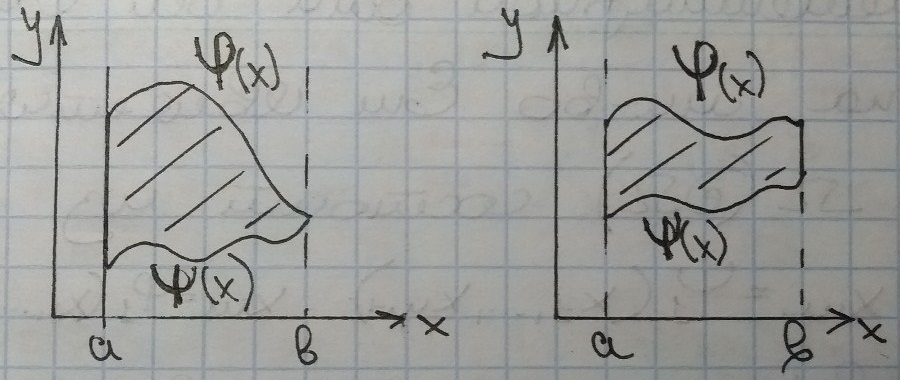
\includegraphics[width=100mm]{lect7pic1}
	\\
=
\end{figure}


\subsection{m-кратные интегралы}


	$\Omega \subset \mathbb{E}^m, \; Ox_1\dots x_m; \;\; \varepsilon_m \{(x_1,\dots, x_m): x_m=0\}$ где $\Omega_m $ - проекция области $\Omega$ на мн-во $\varepsilon_m$
\begin{determenition}
	Область $\Omega\subset \mathbb{E}^m$ называется \textbf{элементарной относительно $Ox_m$}, если ее проекция на $\Omega_m $ на множество $\varepsilon_m$ является областью, а  граница $\Omega$ (т.е.$ \delta\Omega$) состоит из графиков двух функций: $x_m=\phi_1(x_1,\dots, x_{m-1});\; x_m=\psi_1(x_1,\dots, x_{m-1}) $ и, быть может, боковой поверхности цилиндра, основанием которого является $\delta\Omega_m $ причем $\forall (x_1,\dots, x_{m-1})\in \overline{\Omega}_m \rightarrow  \psi(x_1,\dots, x_{m-1}) \leq \phi(x_1,\dots, x_{m-1}).$
	
\end{determenition}

\begin{theorem}
		Пусть $\omega=f(x)$ непрерывна на $\overline{\Omega} $ и область $\Omega$ элементарна относительно оси $Ox_m$, ее граница состоит из двух графиков непрерывных функций $y=\phi_1(x_1,\dots, x_{m-1});$ 
		$ y=\psi_1(x_1,\dots, x_{m-1}) $ и, быть может, боковой поверхности цилиндра оси $Ox_m $,  причем $\forall (x_1,\dots, x_{m-1})\in \overline{\Omega}_m \rightarrow  \psi_1(x_1,\dots, x_{m-1}) \leq \phi_1(x_1,\dots, x_{m-1}).$
	 	Тогда существует повторный интеграл $\underbrace{\int\dots\int}_{\Omega_m} dx_1\dots dx_{m-1} \int_{\psi_1(x_1,\dots, x_{m-1}}^{\phi_1(x_1,\dots, x_{m-1})} f(x) dx_m = \underbrace{\int\dots\int}_{\Omega_m} f(x_1, \dots, x_m)dx_1\dots dx_{m} $\\
	 	$$ \begin{cases}
	 	x=x(u,v) \\ y=y(u,v)
	 	\end{cases} 
	 	(x,y)\in\Omega; (u,v)\in\Omega^*; \; 
	 	\mathbb{J}= 
	 	\begin{vmatrix}
	 		x_u& x_v\\
	 		y_u& y_v
	 	\end{vmatrix};\;\iint\limits_\Omega f(x,y) dxdy=\iint\limits_{\Omega^*}f(x, y) | \mathbb{J}(u,v) | dudv $$
\end{theorem}



\end{document}